\documentclass[11pt]{article}

\usepackage[T1]{fontenc}
\usepackage{librefranklin}
\renewcommand*\familydefault{\sfdefault} %% Only if the base font of the document is to be sans serif


% Margins
 \setlength{\oddsidemargin}{0 in}
 \setlength{\evensidemargin}{0 in}
 \setlength{\textwidth}{6.6 in}
 \setlength{\topmargin}{0 in}
 \setlength{\textheight}{8.55 in}
\setlength{\headheight}{0.18 in}





% Packages  
%\usepackage[margin=0.8 in]{geometry} % decides size of margins, paper etc
%\usepackage{palatino} % a font
\usepackage{hhline}
%\usepackage{forest}
\usepackage{cancel} % to cross out stuff
\usepackage{amsmath}
\usepackage{marginnote}  % to put notes on the margins
\usepackage{amssymb}
\usepackage{amsthm}
\usepackage{accents}
\usepackage{amsfonts}
\usepackage{mathtools}
\usepackage{enumerate}
%\usepackage{verbatim}
\usepackage{comment}
%\usepackage{makeidx}
\usepackage{hyperref}
\usepackage{multirow}
\usepackage[noadjust]{cite}
\usepackage{color}
% \usepackage{pst-node}
% \usepackage{tikz-cd} 
% \usepackage[toc,page]{appendix}			% table of contents


% Global options
\allowdisplaybreaks
\mathtoolsset{showonlyrefs}


% Math Operators
\DeclareMathOperator{\sgn}{sgn}
\DeclareMathOperator{\pv}{pv}
\DeclareMathOperator{\Div}{div}
\DeclareMathOperator{\Int}{int}
\DeclareMathOperator{\dist}{dist}
\DeclareMathOperator{\sech}{sech}
\DeclareMathOperator{\sing}{sing}
\DeclareMathOperator{\supp}{supp}
\DeclareMathOperator{\sign}{sign}
\DeclareMathOperator{\II}{II}
\DeclareMathOperator{\diag}{diag}
\DeclareMathOperator{\trace}{tr}
\DeclareMathOperator{\grad}{grad}
\DeclareMathOperator{\adj}{adj}
\DeclareMathOperator{\Span}{span}
\DeclareMathOperator{\Sym}{Sym}
\DeclareMathOperator{\arcsinh}{arsinh}
\DeclareMathOperator{\artanh}{artanh}
\DeclareMathOperator{\proj}{proj}
\DeclareMathOperator{\arcosh}{arcosh}
\DeclareMathOperator{\Diff}{Diff}

%Special Characters
\let \sectionsymbol \S
\renewcommand{\P}{\mathbb{P}}
\newcommand{\R}{\mathbb{R}}
\newcommand{\B}{\mathbb{B}}
\newcommand{\C}{\mathbb{C}}
\renewcommand{\S}{\mathbb{S}}
\renewcommand{\H}{\mathbb{H}}
\newcommand{\Z}{\mathbb{Z}}
\newcommand{\pr}{\mathcal{p}\mathcal{r}}
\newcommand{\ru}{{\sqrt{u}}}
\newcommand{\SM}{\overline{S^*M}}
\newcommand{\pdo}{\Psi\text{DO}}
\newcommand{\ox}{\o{\xi}}
\newcommand{\tM}{\tilde{M}}
\newcommand{\tg}{\tilde{g}}
\newcommand{\p}{\partial}
\newcommand{\n}{\nabla}
\newcommand{\on}{\overline{\n}}
\newcommand{\tn}{\tilde{\nabla}}
\newcommand{\oM}{\overline{M}}
\newcommand{\tX}{\widetilde{X}}
\newcommand{\ta}{{\widetilde{\alpha}}}
\newcommand{\tx}{{\widetilde{x}}}
\newcommand{\oX}{\overline{X}}
\newcommand{\X}{\mathfrak{X}}
\newcommand{\oW}{\overline{W}}
\newcommand{\oT}{\overline{T}}
\newcommand{\tf}{\tilde{f}}
\newcommand{\tr}{\tilde{\r}}
\newcommand{\x}{{x_c}}
\newcommand{\oU}{\overline{U}}
\newcommand{\oH}{\overline{H}}
\newcommand{\oSU}{\o{S^*U}}
\newcommand{\oSH}{\overline{S^*\mathbb{H}^2}}
\newcommand{\rg}{\rangle}
\renewcommand{\lg}{\langle}
\newcommand{\bTM}{{}^bT^*\oM}
\newcommand{\Di}{\Delta\iota}
\newcommand{\hx}{\hat{\xi}}
\newcommand{\ba}{\breve{a}}
\newcommand{\tz}{\widetilde{\zeta}}
\newcommand{\hY}{\hat{Y}}
\newcommand{\tPhi}{\widetilde{\Phi}}
\newcommand{\og}{\overline{\g}}
\newcommand{\prl}{\parallel}
\newcommand{\cM}{\mathring{M}}


% Calligraphic letters

\newcommand{\calA}{\mathcal{A}}
\newcommand{\calB}{\mathcal{B}}
\newcommand{\calC}{\mathcal{C}}
\newcommand{\calD}{\mathcal{D}}
\newcommand{\calE}{\mathcal{E}}
\newcommand{\calF}{\mathcal{F}}
\newcommand{\calG}{\mathcal{G}}
\newcommand{\calH}{\mathcal{H}}
\newcommand{\calL}{\mathcal{L}}
\newcommand{\calO}{\mathcal{O}}
\newcommand{\calR}{\mathcal{R}}
\newcommand{\calS}{\mathcal{S}}
\newcommand{\calU}{\mathcal{U}}
\newcommand{\calV}{\mathcal{V}}
\newcommand{\calW}{\mathcal{W}}
\newcommand{\calY}{\mathcal{Y}}
\newcommand{\calZ}{\mathcal{Z}}


%Greek Letters

\renewcommand{\a}{\alpha}
\renewcommand{\b}{\beta}
\newcommand{\g}{\gamma}
\renewcommand{\d}{\delta}
\let\epsilon\varepsilon
\newcommand{\e}{\epsilon}
\newcommand{\h}{\eta}
\newcommand{\z}{\zeta}
\newcommand{\smsec}{\G_0^{\frac{1}{2}}}
\newcommand{\G}{\Gamma}
\newcommand{\oG}{\overline{\Gamma}}
\renewcommand{\r}{\rho}
\renewcommand{\t}{\tau}
\renewcommand{\k}{\kappa}
\renewcommand{\l}{\lambda}
\newcommand{\s}{\sigma}
\renewcommand{\th}{\theta}
\newcommand{\om}{\omega}
\newcommand{\w}{\omega}
\renewcommand{\oe}{\overline{\eta}}
\newcommand{\tU}{\tilde{U}}

% Environments

\newtheorem{definition}{Definition}
\newtheorem{lemma}{{Lemma}}
\newtheorem{theorem}{Theorem}
\newtheorem{proposition}{Proposition}
\newtheorem{conjecture}{Conjecture}
\newtheorem{remark}{Remark}
\newtheorem{corollary}{Corollary}
\newtheorem{example}{Example}
\newtheorem{ansatz}{Ansatz}
\newtheorem{problem}{Problem}
\newtheorem{question}{Question}
\newenvironment{solution}{\paragraph{Solution:}}{\hfill$\square$}
\newtheorem{goal}{Goal}
\newtheorem{claim}{Claim}
\newtheorem{idea_that_doesnt_work}{Idea that doesn't work}
\newtheorem{unverified_claim}{Unverified Claim}
\newenvironment{answer}{\paragraph{Answer:}}{\hfill$\square$}


\let \o \undefined
\def \o#1{\overline{#1}}
\def\fr#1#2{\frac{#1}{#2}}
\def\tt#1{\textit{#1}}

% \let\printintex\undefined
% \let\see\undefined

\let\td\undefined
\def \td#1{\widetilde{#1}}
\let\implies\Rightarrow


\author{Nikolas Eptaminitakis}


\usepackage{enumitem}

\begin{document}
\section*{Nonlinear Mechanical Systems Worksheet}

\subsection*{Spring-mass systems}

The purpose of the first part of this worksheet is to understand spring-mass systems in which the spring force is not given by the usual linear Hooke's law $F(x)=-kx$, where $k>0$ is the spring constant and $x$ the displacement from equilibrium, but by a nonlinear function of $x$.
One of the simplest forms of nonlinear spring force we consider is
\begin{equation}
	F(x)=-kx+\b x^3,
\end{equation}
where $\b\neq 0 $ is a constant.
The equation of damped motion for the object of mass $m$ becomes 
\begin{equation}
	mx''+cx'=-kx+\b x^3.\label{eq:motion}
\end{equation}
The spring is called \textit{hard} if $\b<0$ and \textit{soft} if $\b>0$. The constant $c>0$ is the damping constant.
\begin{enumerate}
	\item \label{p1} Rewrite \eqref{eq:motion} as an equivalent 1st order system for the displacement and velocity.
	\item \label{p2} Suppose that $m=1$, $k=4$, $c=0$ and $\b=-1$ (hard spring). 
	\begin{enumerate}
		\item Find the critical points of the system in Part \ref{p1}. Are they isolated?
		\item Compute the linearization of the system at each critical point. Determine the type (spiral, center etc) and stability properties of the linearized system. 
		\item What can you say about the type and stability of the nonlinear system at each of the critical points?
	\end{enumerate}
	\item Do the same as in part \ref{p2} but for a soft spring and with damping: take $m=1$, $k=4$, $c=1$ and $\b=1$.

	\item Which of the phase plane portraits below corresponds to the soft spring with damping and which one to the hard spring? Notice how different the trajectories are!

	\begin{figure}[h]
		\minipage{0.32\textwidth}
		  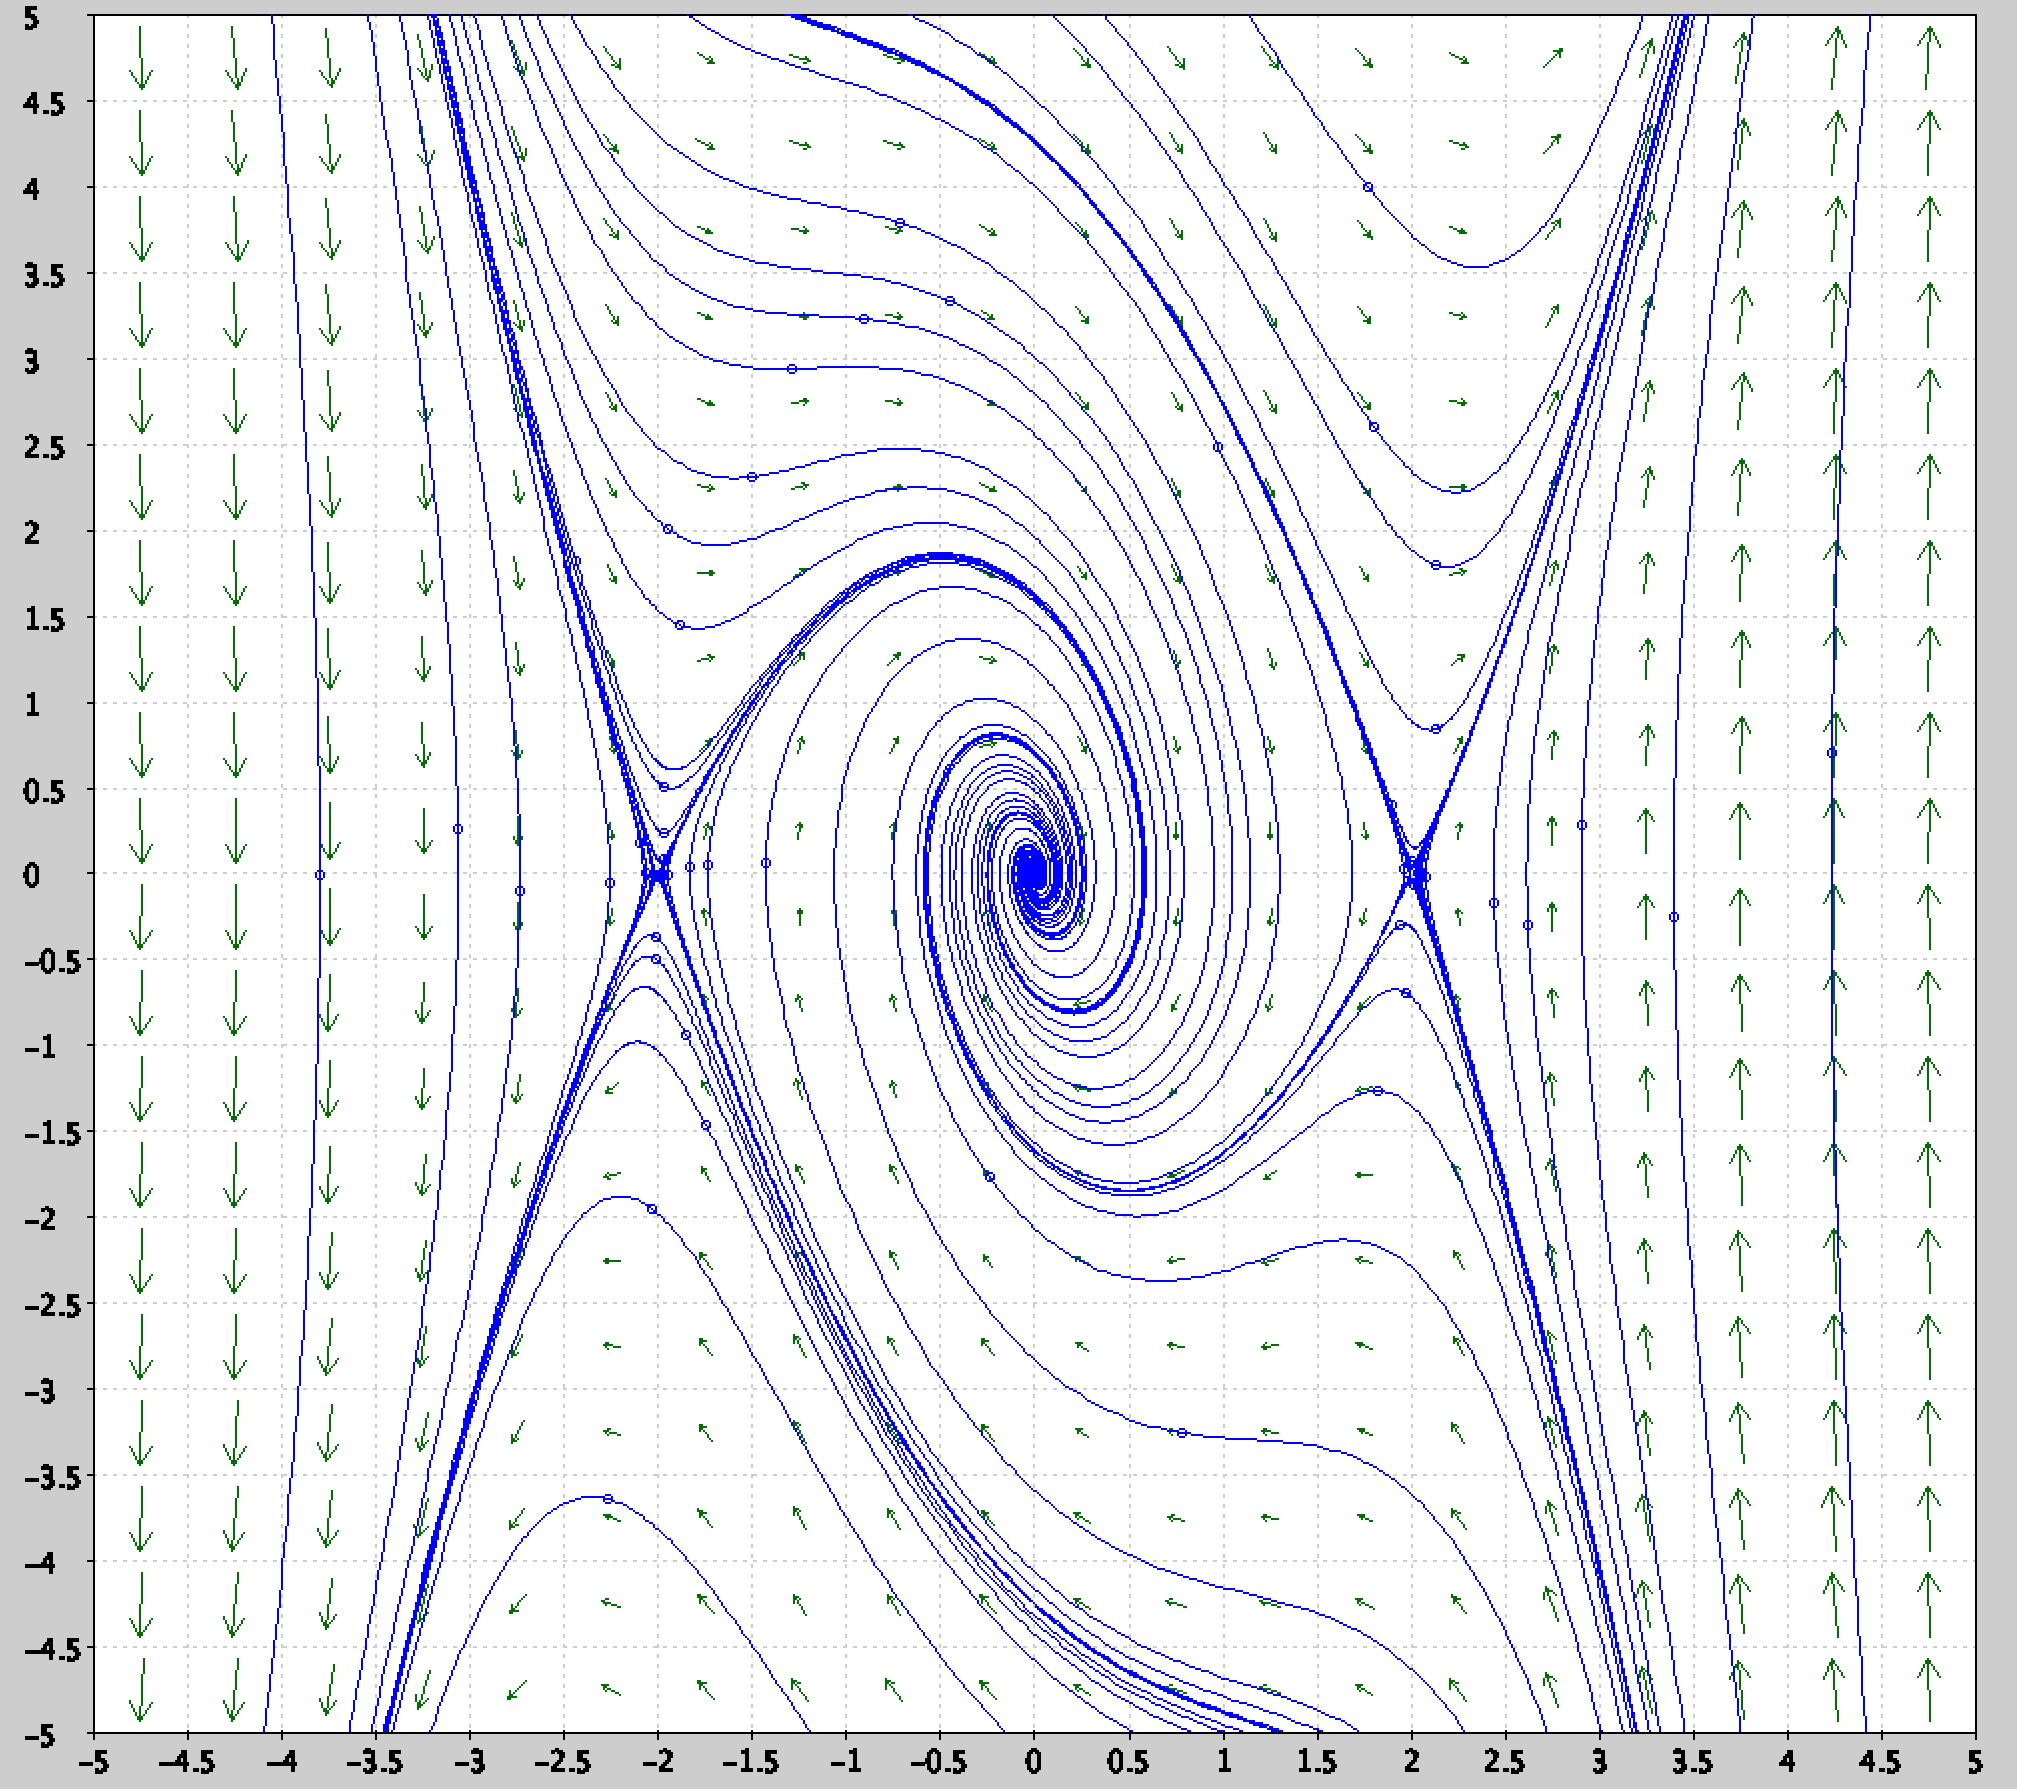
\includegraphics[width=\linewidth]{figA}
		  \caption{A}
		  % \label{}
	\endminipage\hfill
		\minipage{0.32\textwidth}
		  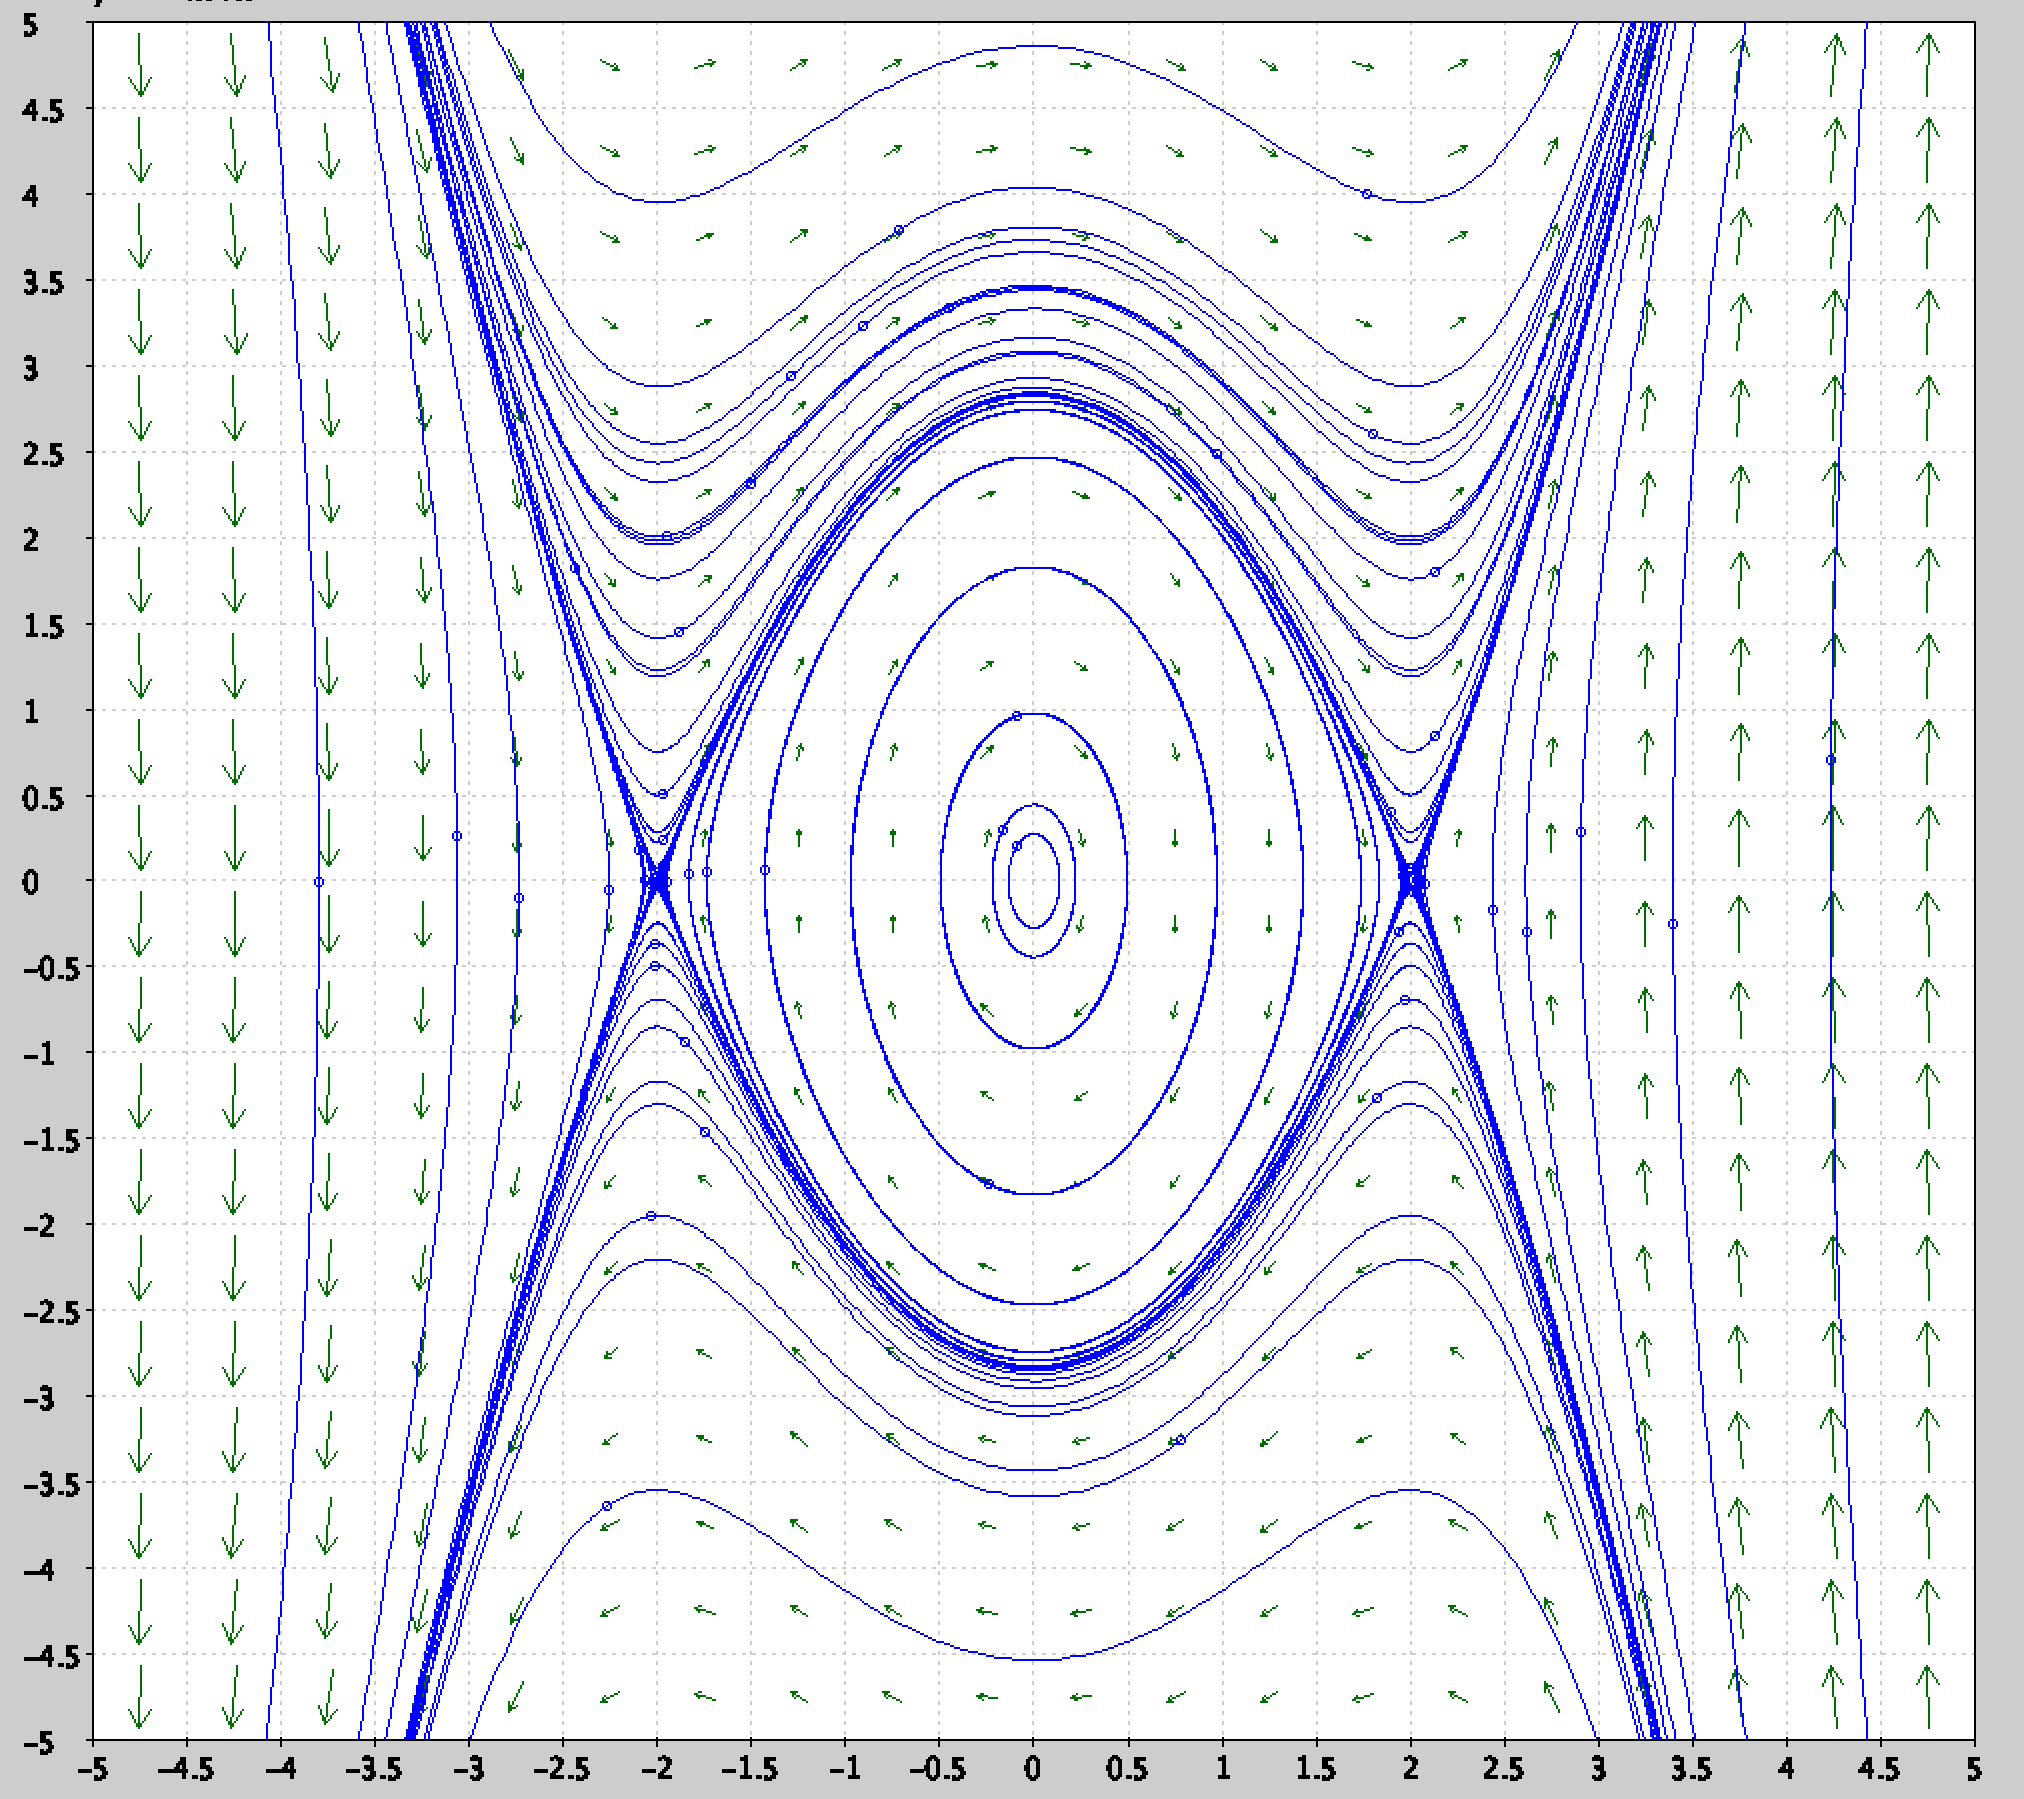
\includegraphics[width=\linewidth]{figB}
		  \caption{B}
		  % \label{}
	\endminipage\hfill
		\minipage{0.32\textwidth}
		  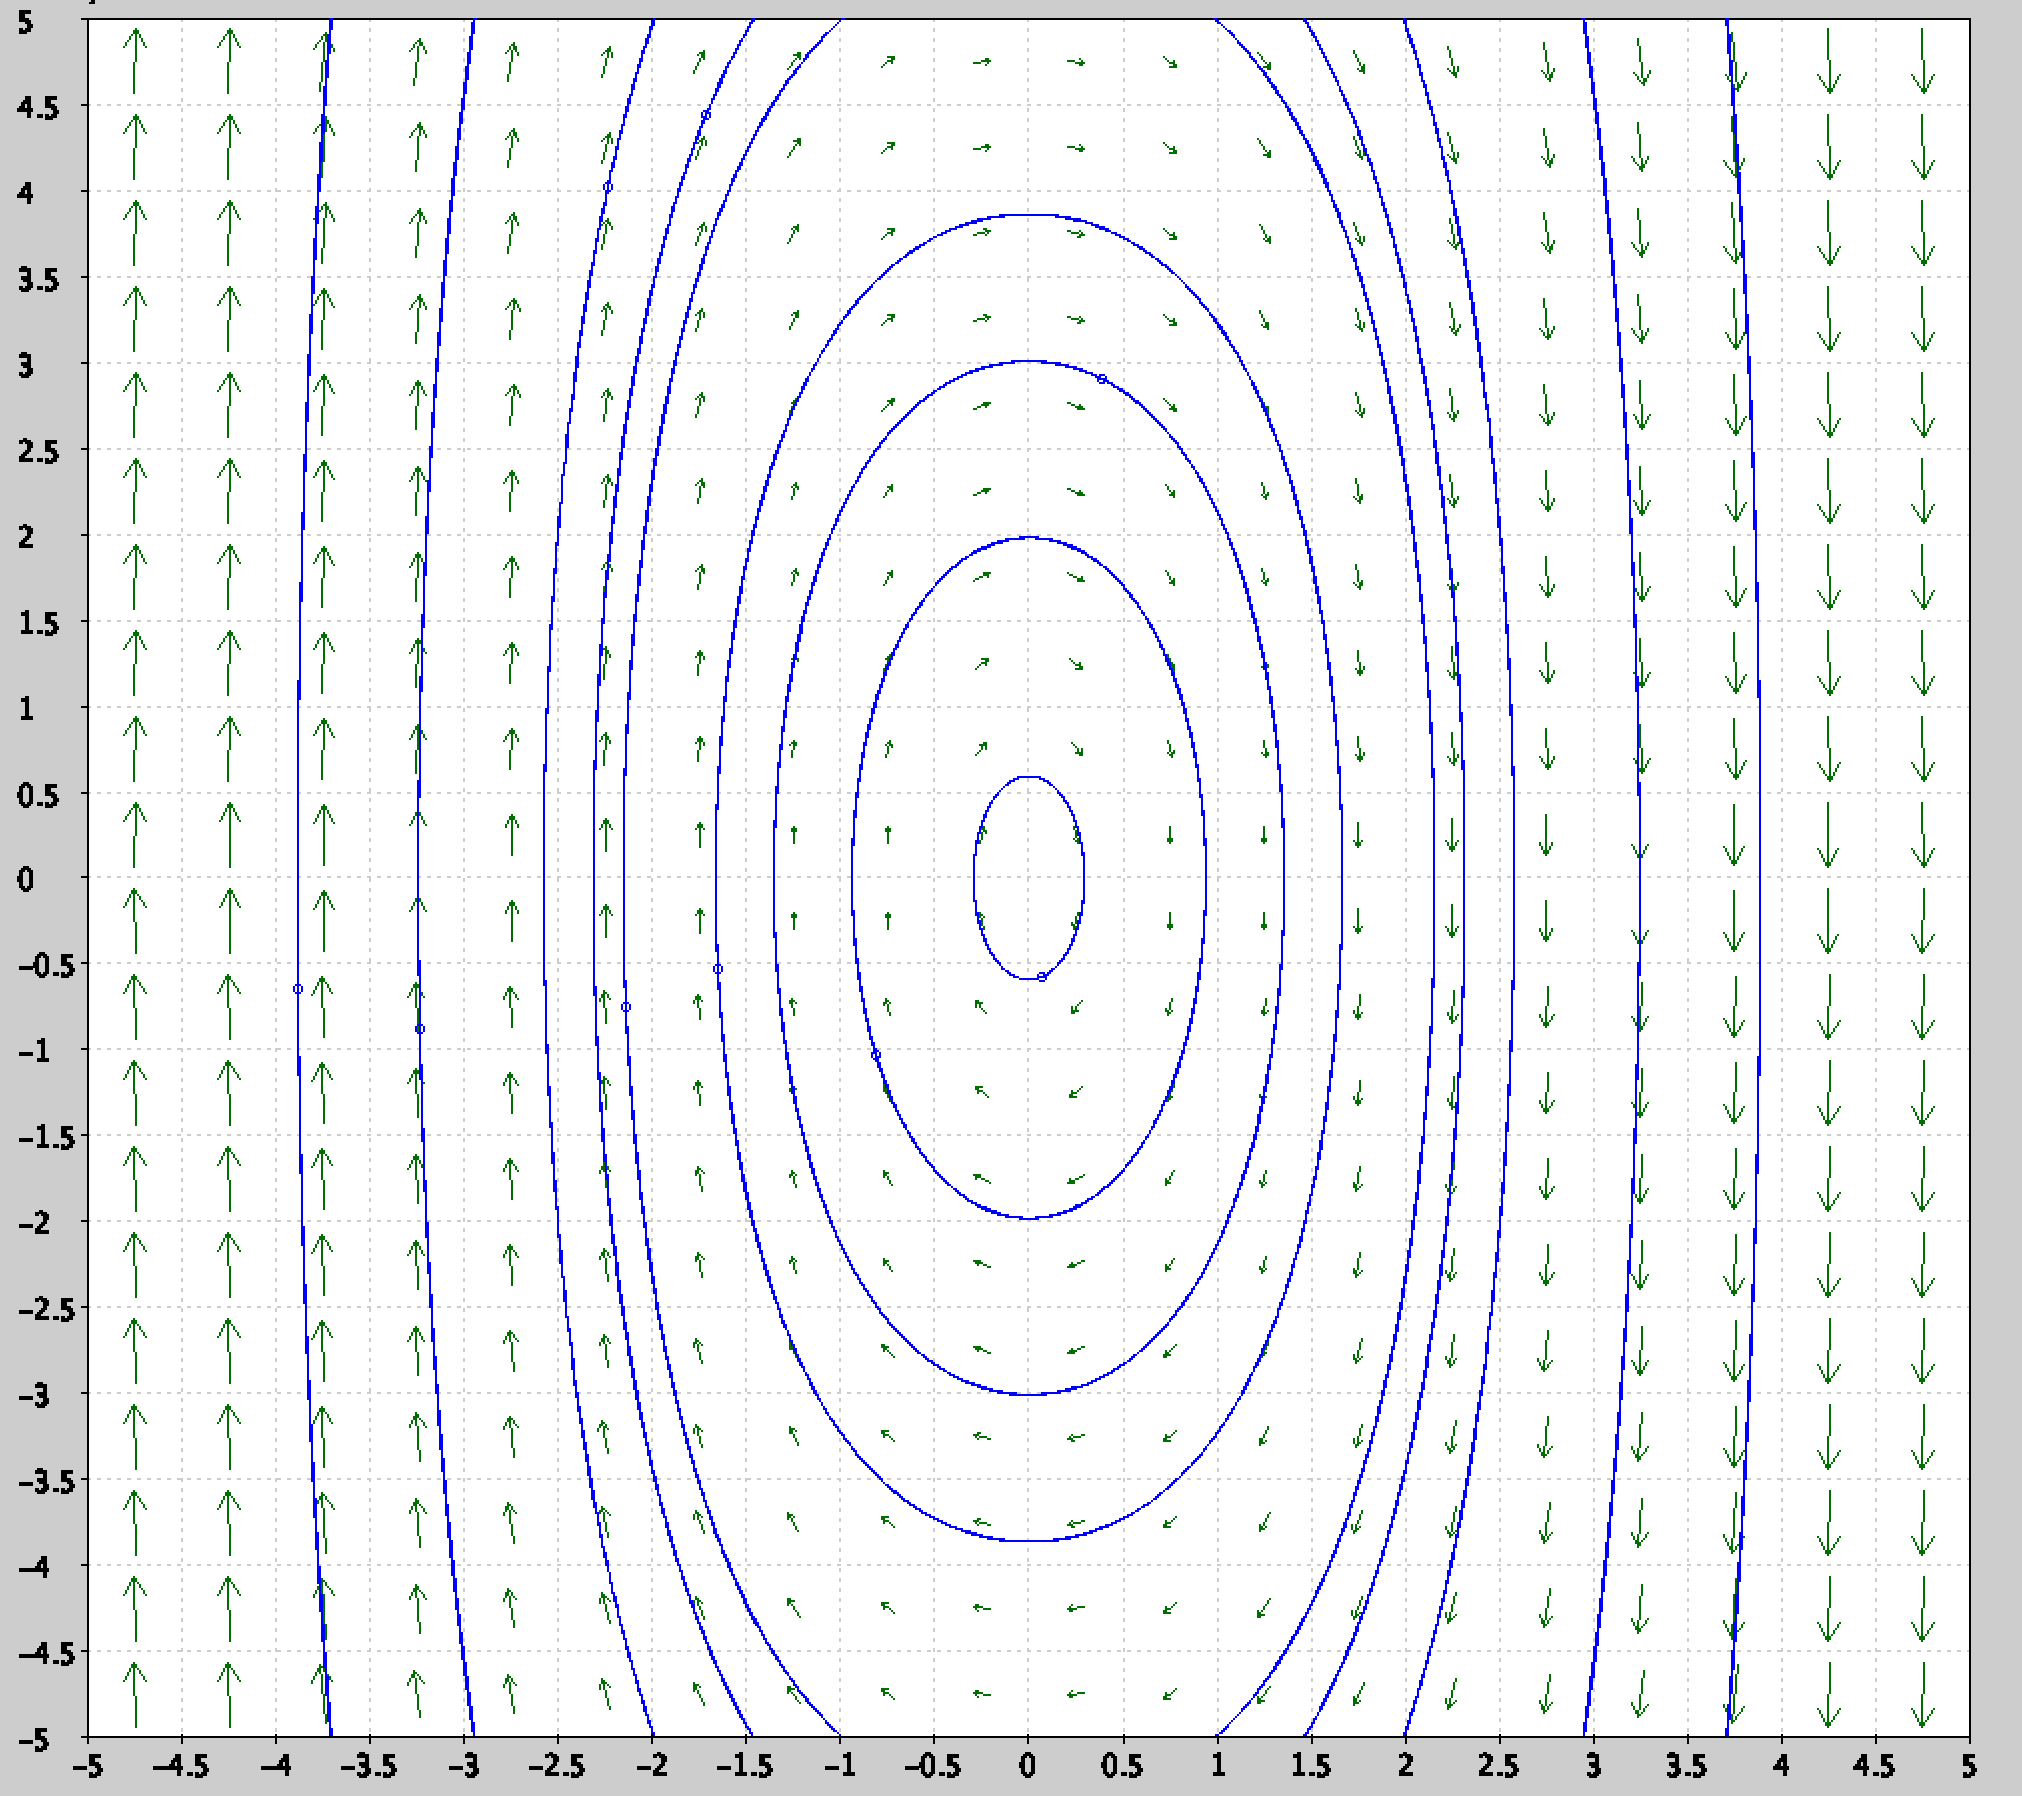
\includegraphics[width=\linewidth]{figC}
		  \caption{C}
		  % \label{}
		\endminipage
	\end{figure}



	\item * You can say more about the trajectories near a center in the following way: Look at the example in Part \ref{p2}: recall from calculus that along a curve $(x(t),y(t))$ with $x'(t)\neq 0$ we can write $$\frac{dy}{dx}=\frac{y'(t)}{x'(t)}.$$
	Then use the equations in your system from part \ref{p1} to reach a differential equation of the form $\frac{dy}{dx}=f(x)g(y)$, that is, a separable first order differential equation for $y=y(x)$. 
	Now separate variables to solve it. In this way you can obtain an implicitly defined formula for the trajectories.
\end{enumerate}






\subsection*{Nonlinear Pendulum}
The equation for the nonlinear pendulum with damping is given by 
\begin{equation}\label{pendulum}
	\frac{d^2\th}{dt^2}+c\frac{d\th}{dt}+\w^2\sin\th=0,
\end{equation}
where $\w^2=g/L$ with $g$ the gravitational constant, $L$ the length of the massless rod, $c>0$ is the damping constant, and $\th$ the angle with the vertical axis (see Fig. \ref{fig:pendulum}).
(For a derivation of \eqref{pendulum} see Section 3.4 in the textbook.)
\begin{enumerate}[resume]
	\item Rewrite \eqref{pendulum} as an equivalent first order system
	\item From now on consider the case $c=0$ and $\w=1$. Find its critical points. Are they isolated?
	\item  Compute the Jacobian matrix at the critical points and its eigenvalues. What can you say about the type of the critical points and their stability?
	\item The phase plane portrait for this system is seen below. Describe physically the behavior of the mass attached to the pendulum if its initial conditions are at each of the three points $A$, $B$, $C$ below:
	
	\begin{figure}[h]
    	\centering
	    	\parbox{5cm}{
	    	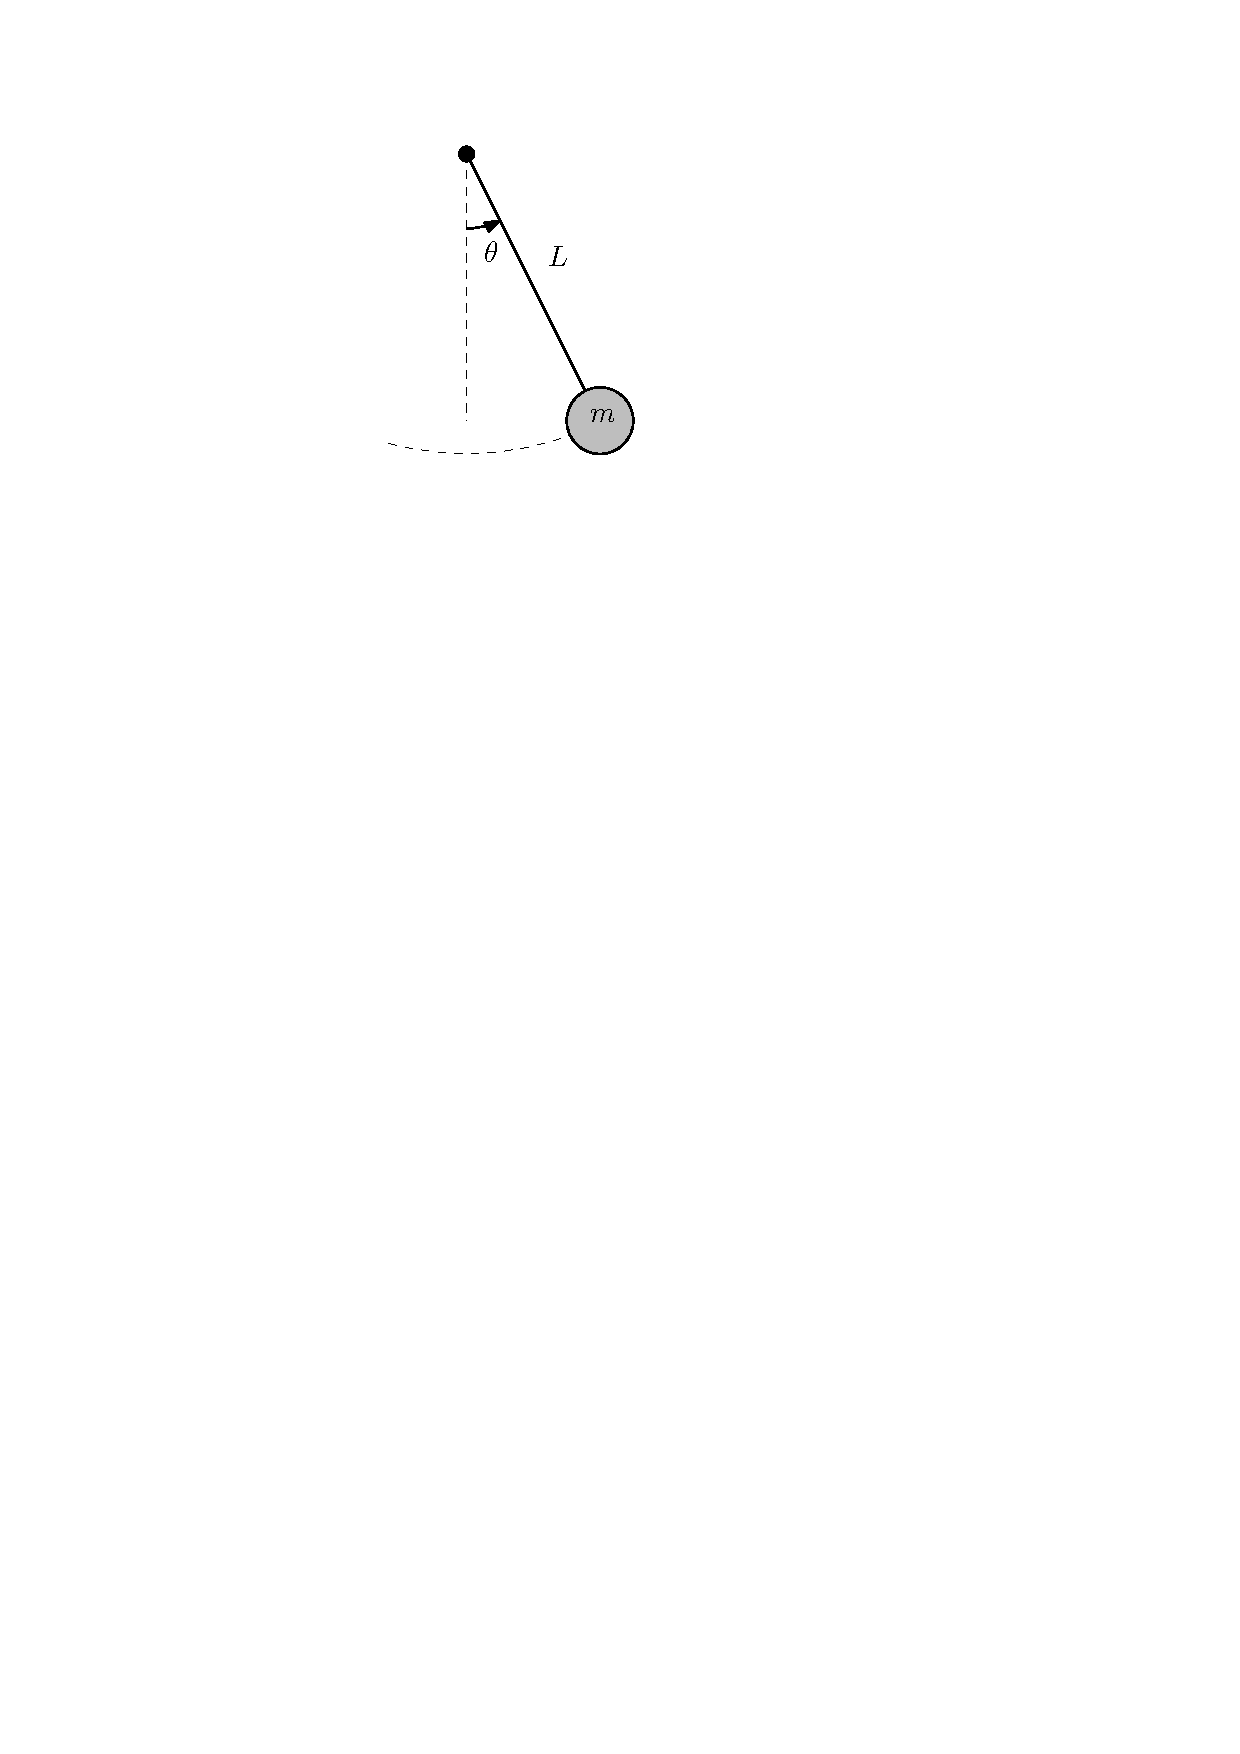
\includegraphics[scale=.7]{Pendulum.pdf}
	    	\caption{Pendulum}
    	\label{fig:pendulum}}
    	\qquad
		    \begin{minipage}{5cm}
		    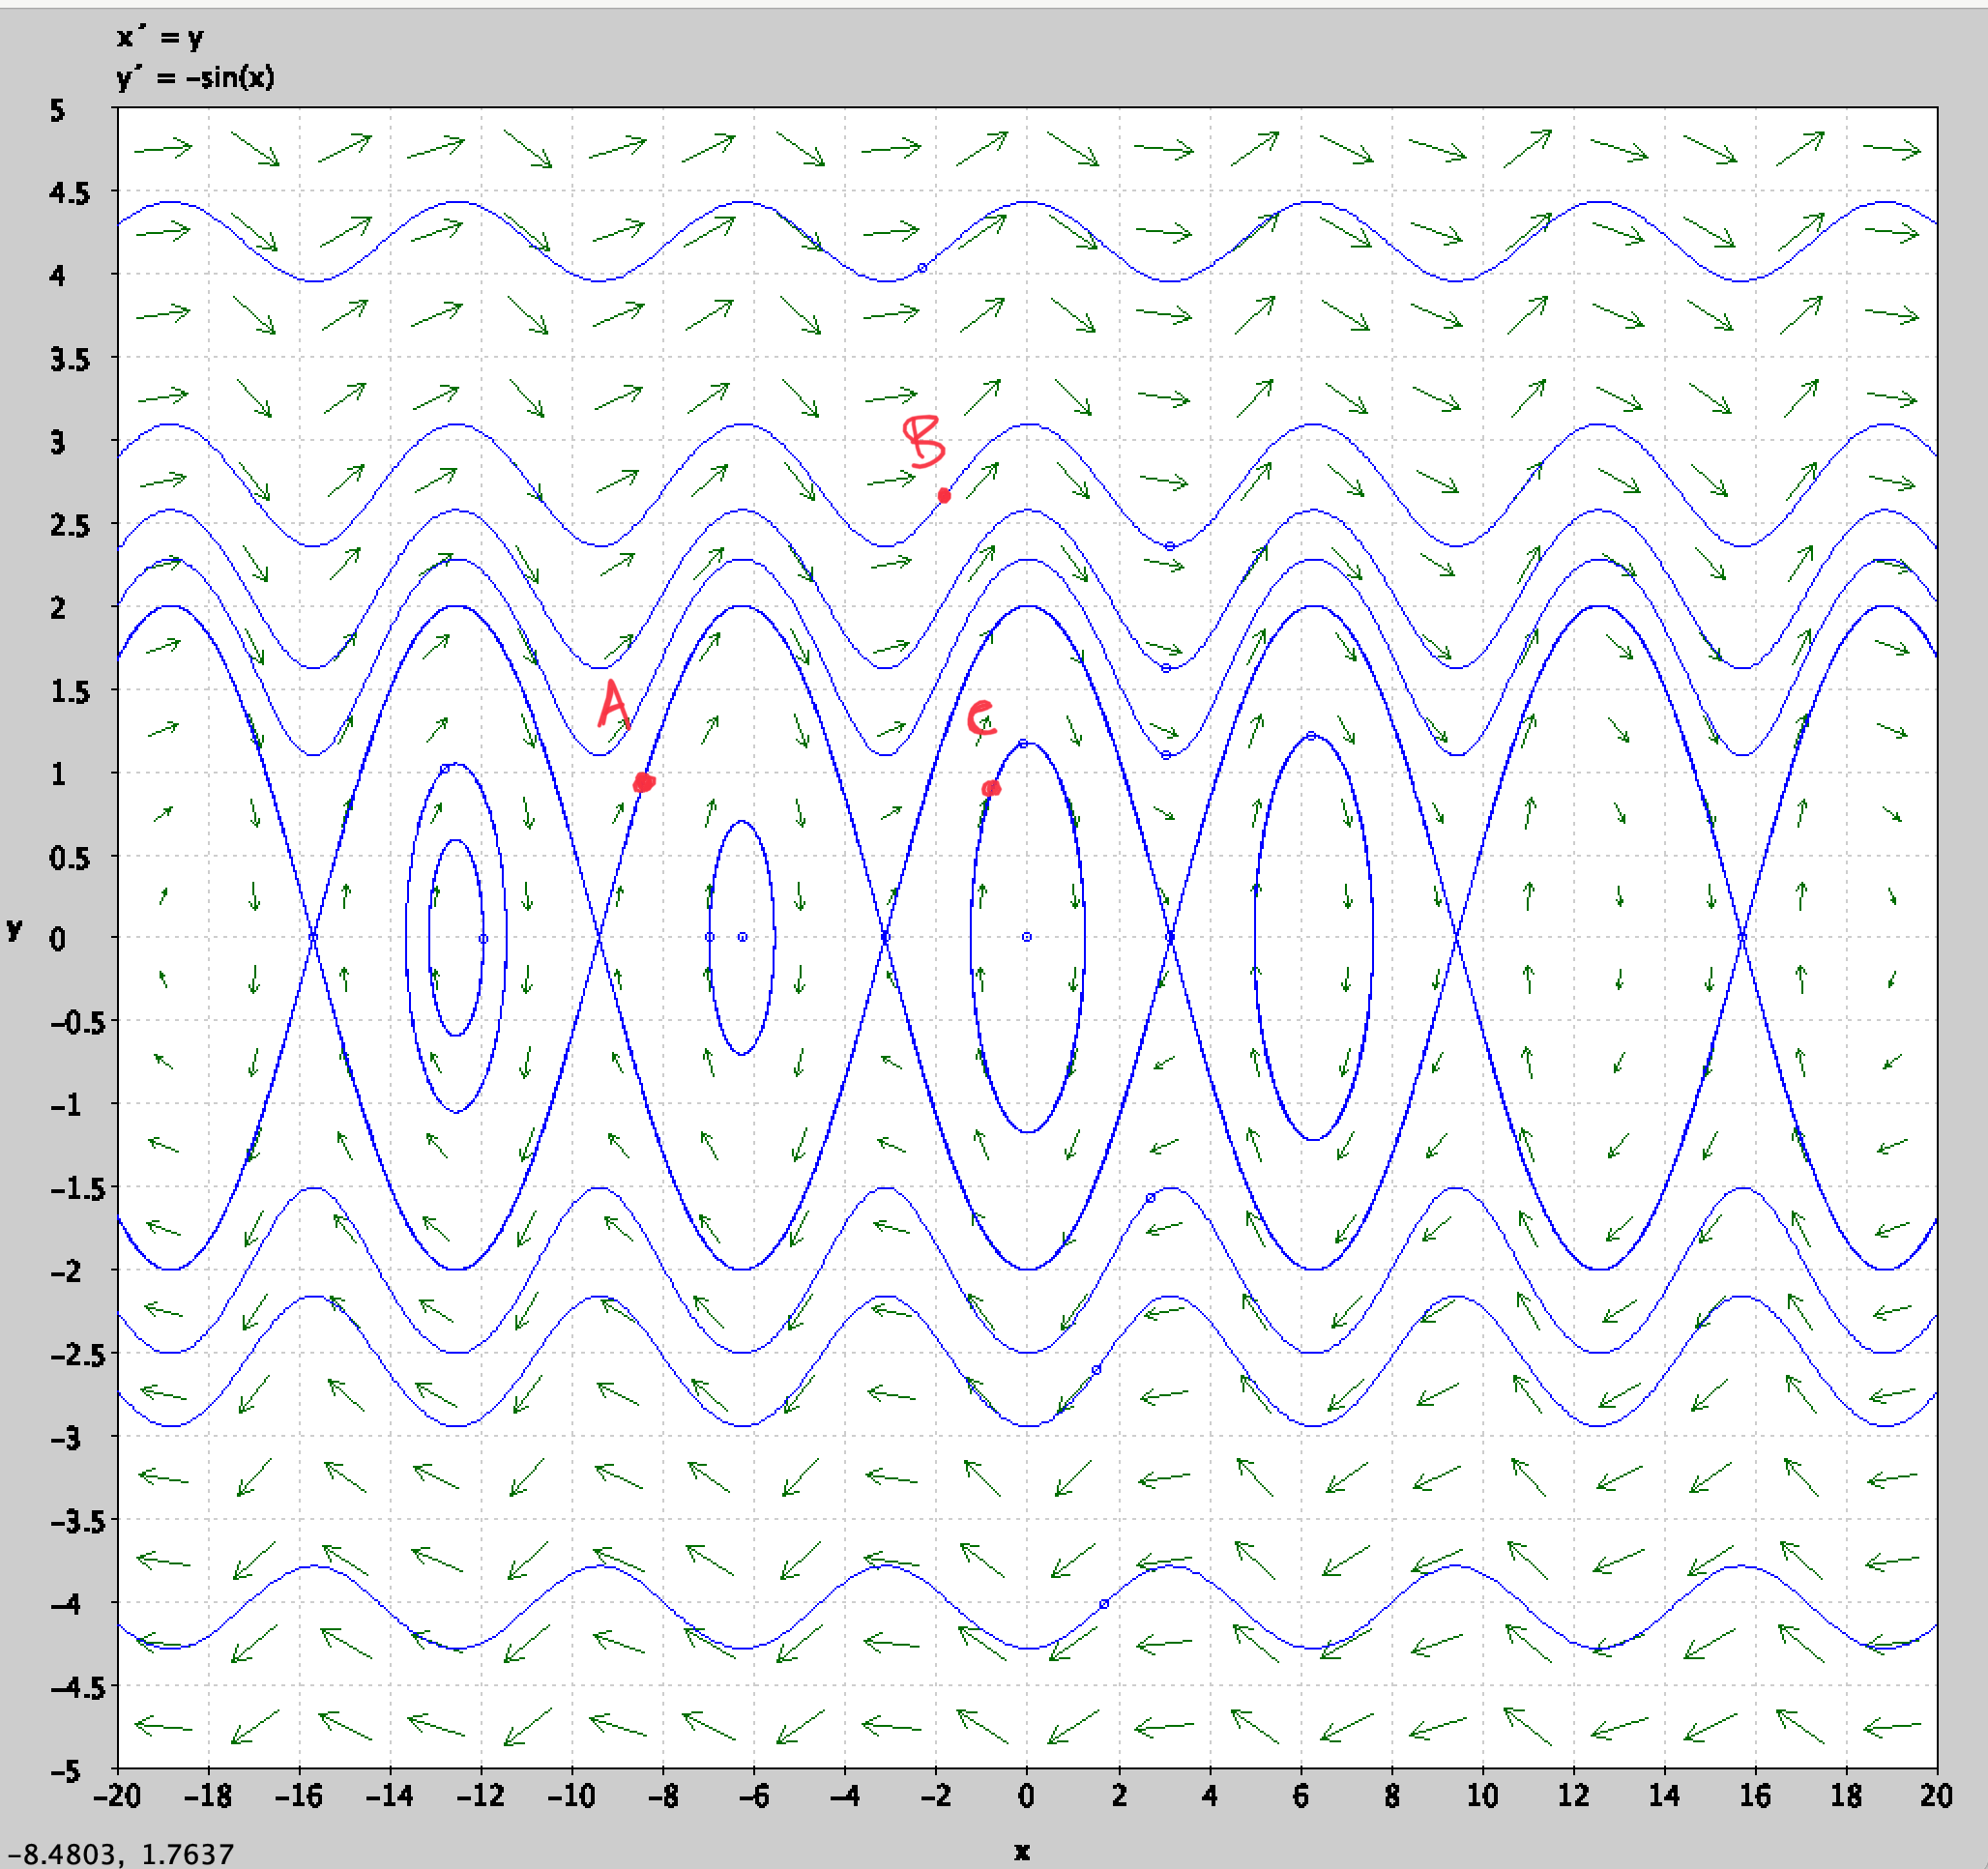
\includegraphics[width=6 cm]{pendulum.png}
		    \caption{Phase Plane Portrait}
		    \label{}
	    \end{minipage}
    \end{figure}
		
\end{enumerate}























\end{document}